\documentclass[ebook,12pt,oneside,openany]{memoir}
\usepackage[utf8x]{inputenc}
\usepackage[english]{babel}
\usepackage{amsmath,amssymb,amsfonts,amsthm}
\usepackage{graphicx}
\usepackage{microtype}
\usepackage{enumitem}
\usepackage[listings,theorems]{tcolorbox}
\usepackage{hyperref}
\hypersetup{
    colorlinks = true,
    urlcolor = violet,
    linkcolor = blue,
}
\setlength{\parindent}{4em}
\setlength{\parskip}{1em}
\renewcommand{\baselinestretch}{1.2} 
\addto\captionsenglish{\renewcommand*\contentsname{Table of Contents}}

\title{\underline{\textbf{Liquid Drop Model}}}
\author{Durjoy Dutta Chaudhury}
\date{2021}



\begin{document}

\maketitle

\pagebreak

\tableofcontents
\listoffigures
\listoftables




\chapter{Liquid Drop Model} 
 
     \begin{tcolorbox} [title = \textbf{Key Objectives:}, width = \textwidth]
    Liquid Drop Model
    \begin{itemize}
        \item Nuclear Landscape
        \item Liquid drop model
        \item Similarity \& limitations
        \item Bethe–Weizsäcker mass formula \\ (Semi-empirical mass formula) 
    \end{itemize}
    \end{tcolorbox}
 
    \section{Nuclear Landscape}
    Our knowledge of the nuclear force gives us understanding about the formation of nuclei. There are about 3300 nuclei known to us but only a fraction of them are stable! In fact, it is around only 15\% of the total list. Most of the unstable (radioactive) nuclei undergo -decay and few, mostly the heavy nuclei decay through  particle emission. Some of the heavy nuclei also undergo spontaneous fission (breaking of a nucleus into two lighter nuclei). This can be clearly seen in the Z vs N plot from figure \ref{fig:plot_ZvsN} which is also known as Segre chart (\href{https://www.nndc.bnl.gov/nudat2/}{link for more info.}) of all the known nuclei.
    
        \begin{figure}
            \centering
            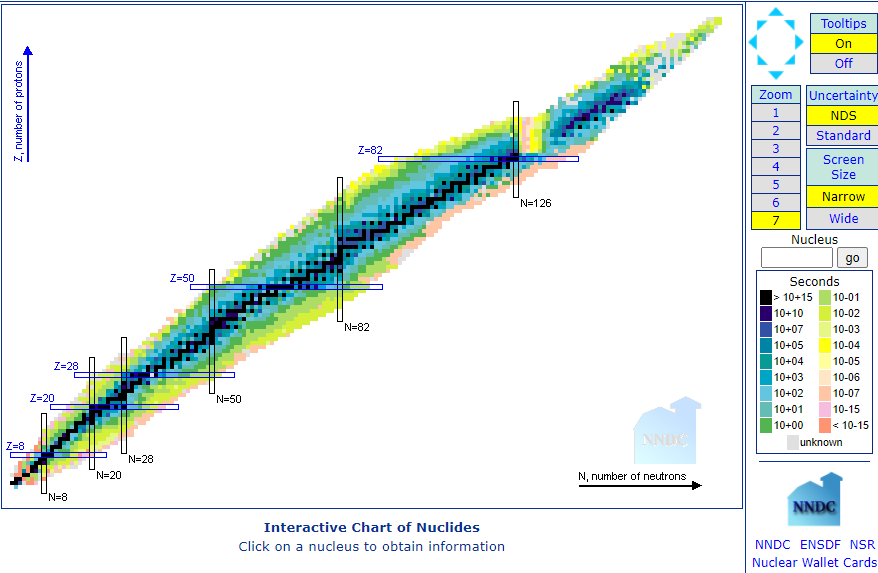
\includegraphics[width = \textwidth]{images/ZvN_plot.png}
            \caption{Z vs N Plot}
            \label{fig:plot_ZvsN}
        \end{figure}
    
    \par The black dots in the plot are the stable nuclei whereas the other colours correspond to unstable nuclei with varying half-life (range is given in the box). It shows that as we move toward the heavier nuclei, it needs more neutrons than protons to stabilize a nucleus. This observation seemingly contradicts the charge symmetry of the nuclear force! However, it may be explained as the effect of Coulomb repulsions between the protons which weaken the binding energy of a nucleus. To compensate for this loss, more and more neutrons are needed in heavier nuclei. At this point if we recollect our lessons from B.E./A systematics, we have seen that even-even (both N and Z are even) nuclei are strongly bound compared to their odd-odd neighbours with same A (isobar). Similarly, for isotopes (nuclei with same Z) and isotones (nuclei with same N), it has been observed that odd-even or even-odd combinations are relatively stronger bound than neighbouring odd-odd combinations and weakly bound with respect to even-even neighbours. This tells us apart from the attractive short range interaction and Coulomb force, there are other components in the nuclear force. In this class, we will develop a phenomenological (Semi-empirical) model of the nucleus as functions of A, Z and N using existing knowledge of the nuclear force and features of binding energy.
    \par The above discussion must have triggered an intriguing question in your mind: what is the difference between an even-even and an odd-odd nucleus from the nuclear force aspect? In fact there should not be any! The answer lies in the fact that the exact form of the nucleon-nucleon interaction is still not known to us. There are many components in it and not necessarily all of them will help in increasing binding energy of a nucleus. It is further to be noted that even if we know the exact form of the potential, we can not solve the corresponding Schrodinger equation exactly due to the presence of three body components in the nucleon-nucleon interaction to a many body system. Exactly at this point the nuclear physics, low energy nuclear physics to be precise, differs from the atomic physics which can be solved exactly with the electro-magnetic interaction which is exactly known to physicists. This led to the development of a model to explain the observed features. The known properties of the nuclear force will act as the input to the model.
    
    
        \subsection{What is a model in science?}
        A scientific model is a conceptual representation of a system to understand, visualize, or simulate the system using the accepted knowledge. Usually, a model is bound by strict assumptions and intends to describe a few particular features of the system. Therefore, no model intends to give a full description of the system from all angles but to explain a few features. 

    \section{Liquid Drop Model}
    This model was first proposed by N. Bohr and F. Kalcker in 1937. Later it was refined and applied by C. F. von Weizsäcker and H. Bethe to develop the semi-empirical mass formula (also known as \textbf{Bethe–Weizsäcker mass formula}) as mentioned above.  The model has been very useful for the understanding of nuclear fission data and predicting the masses and stability of a nucleus based on the Strutinsky method. The analogy between the charged liquid drop and atomic nucleus can was made based on the following similarities:
    
        \begin{itemize}
        
            \item Similarity:
            
                \begin{enumerate}
                    \item Like nucleons, molecules in liquid drop also interact with the other molecules in their immediate neighbourhood. Therefore, the interaction between the molecules in a liquid also exhibits saturation properties. Thus, the number of molecules (A) in a liquid drop $\propto$ its volume (V). This can be alternatively established as the total heat required to evaporate a drop of liquid is linearly proportional to the number of molecules in the drop. It is analogous to the total binding energy of a nucleus which is proportional to the number of nucleons in that nucleus.
                    \item Like nucleons, the intermolecular force in a liquid is repulsive at short distances and attractive at intermediate distances and negligible at large distances.
                    \item Like a nucleus, a liquid drop is also nearly incompressible.
                    \item Nucleons near the surface of the nucleus feel less interaction like the surface tension effects observed in liquid drop.
                    \item The internal energy of a nucleus is analogous to the internal thermal vibrations of molecules in the liquid.
                    \item Emission of $\alpha$, $\beta$, p and n may be compared with the evaporation of molecules from liquid.
                \end{enumerate}
            
            \item Limitations:
                \par It is to be noted that there are also striking similarities between a charged liquid drop and an atomic nucleus (which must be quite obvious to you). These are as follows:
            
                \begin{enumerate}
                    \item The foremost difference is that the motion of the nucleons inside a nucleus is of quantum mechanical character whereas the motion of molecules in a liquid is classical in nature.
                    \item Intermolecular attraction acts beyond the dimensions of the electron shells. They also strongly repel each other once the distance is smaller than the size of the electron orbits. On the contrary, nuclear force is attractive within the smaller range, the range of the nuclear forces.
                    \item The average kinetic energy of the molecules in the liquid is $\sim0.1$ eV which corresponds to the de-Broglie wavelength of $\sim10^{-11}$ eV. The average kinetic energy of the nucleons in nuclei is $\sim10$ MeV and it corresponds to the de-Broglie wavelength $\sim10^{-15}$ m order of inter-nucleon distances.
                \end{enumerate}
        \end{itemize} 
        
    Based on the above similarities between the charged liquid drop and atomic nucleus, the liquid drop model was developed. We know that the binding energy ($E_B$) of a nucleus with atomic mass M(A, Z) may be written as
        \begin{equation}
        E_B = ZM_H + NM_n - M(A, Z)
        \end{equation} 
    \par In a phenomenological model, we add different components by hand based on our experimental observation. Let us approach in the same way with our knowledge about $E_B$ as follows:
    
    
    \begin{enumerate}[label=\textbf{\Alph*.}]
    
        \item \textbf{Volume term:}     If we apply our knowledge of nuclear force, the most powerful component would be the attractive short range nuclear force which is proportional to the volume of the nucleus. This term, known as volume energy ($E_v$), obviously favours the binding energy and, thus, is considered positive. It may be written as
        
            \begin{equation}
                \begin{split}
                    E_v &\propto V\\
                    E_v &\propto A = a_VA
                \end{split}    
            \end{equation}
            \hspace{5em} where $a_V$ is the constant of proportionality.
    
        \item \textbf{Surface term:}    Each nucleon interacts with a fixed number of nucleons and it is independent of A. This is the core concept of the volume energy term. However, this is not true for the nucleons on the surface of the nucleus which have less number of neighbouring nucleons. Therefore, the second term, which is known as the surface energy ($E_s$), is a correction to the volume term and should be subtracted from the volume term. It is proportional to the surface area of the nucleus and can be written as:
            \begin{equation}
                \begin{split}
                    E_s &\propto -4\pi R^2 \propto -4 \pi (r_0A^{1/3})^2\\&\propto -4 \pi r_0^2 A^{2/3}\\
                    E_s &= -a_sA^{2/3}
                \end{split}
            \end{equation}
        
        \item \textbf{Coulomb term:}    The protons inside a nucleus repel each other and decrease the overall binding energy. Thus, the Coulomb term is subtracted from the volume term. We can calculate the Coulomb potential energy inside a nucleus assuming that the nucleus is modeled as a uniformly charged sphere of radius $R$ and total charge $Ze$.  The potential energy of the charge distribution may be written as:
            \begin{equation}
                E_C = -\frac{1}{4 \pi \epsilon_0}  \int_0^{Ze} \frac{Q(r)}{r}dQ
            \end{equation}
        
            \hspace{5em} Where $Q(r)$ is the total charge inside a sphere of radius $r$, $dQ$ is infinitesimal small charge at distance $r$ from the center of the sphere. Therefore,
            \begin{align}
                Q~=~Ze(r/R)^3~~\textrm{and}~~dQ~=~\frac{3Zer^2}{R^3}dr\\
                \therefore E_C~=-~\frac{1}{4 \pi \epsilon_0}~\int_0^R \frac{3(Ze)^2}{r} \frac{r^5}{R^6}dr ~~=~-~\frac{3}{5} \frac{(Ze)^2}{4 \pi \epsilon_0 R}
            \end{align}
        
            \hspace{3em} In this calculation, we didn’t rule out the self interaction of the proton. In order to exclude this ambiguity $(Ze)^2$  should be replaced by $Z(Z-1)e^2$ .
            \begin{multline*}
                E_C~=~-\frac{3}{5} \frac{Z(Z-1)e^2}{4 \pi \epsilon_0 R}\\ ~=-~\frac{3}{5} \frac{Z(Z-1)e^2}{4 \pi \epsilon_0 r_0 A^{1/3}}\\ = - a_C \frac{Z(Z-1)}{A^{1/3}}
            \end{multline*}
            \begin{quote}Please note that for large  value, you may write $Z-1 \approx Z$.\end{quote}
            
            Note that the above deduction is not exact. One needs to consider at least
            \begin{itemize}
                \item The effect of departure from the spherical shape of the nucleus
                \item The effect of non-uniform charge density inside the nucleus.
            \end{itemize}
            However, detailed discussions on these effects are beyond the scope of the present syllabus.
            
        \item \textbf{Asymmetry term:}  Heavier nuclei contain more neutrons than protons to compensate for the Coulomb repulsion through more attractive short range interaction. However, adding more neutrons indicates that they will occupy higher energy states, resulting in an increase in the total energy of the nucleus. If we are able to switch off the Coulomb repulsion, the most stable condition would be $N = Z$. This is exactly what we observe in the lighter nuclei where combination gives the most stable isotopes for any given $A$. Therefore, departure from $N = Z$ configuration decreases the binding energy of a nucleus. This asymmetry term may be written as:
        
            \[E_A~=~-a_A\frac{(A-2Z)^2}{A}\]
            \hspace{3em} In this form, the asymmetry term becomes zero when $A = 2Z$. A in the denominator ensures that this effect is less for larger $A$ and vice-versa.
            
        \item \textbf{Pairing term:}    This is the last term in the\\\textit{Bethe–Weizsäcker mass formula}. This term mimics the effect of spin-coupling. We have learned that the ground state \href{https://en.wikipedia.org/wiki/Spin_(physics)}{spin} of all the even-even nuclei are \href{https://drive.google.com/open?id=18RsdVErJJl_99e-parV5QwhS9Gux2CG35fvEiPZISR0}{$0\pm$} which indicates that like-nucleons tend to pair off. It means that in even-even nuclei all the neutrons and all the protons are paired which is a favourable condition to have larger binding energy. For odd-$A$ nuclei, either one proton or one neutron left out without pairing. However, for odd-odd nuclei, one proton and neutron are left unpaired and, thus, contributes least in the binding energy of a nucleus. Mathematically this effect is expressed as:
        
            \begin{equation}
                \begin{split}
                    \delta(A,~Z)~&=~+\delta,~ \textrm       {for N and Z even (even A)}\\
                    \delta(A,~Z)~&=~0,~ \textrm             {for odd A}\\
                    \delta(A,~Z)~&=~-\delta,~ \textrm       {for N and Z odd (even A)}\\
                \end{split}
            \end{equation}
            
            \begin{figure}
                \includegraphics[width = \textwidth]{images/BE_A_plot.png}
                \caption{B(A,Z)/A plot as function of A. The contribution of different terms of Bethe-Weizsäcker mass formula.\\Source: MIT Open Courseware: \href{https://ocw.mit.edu/courses/nuclear-engineering/22-02-introduction-to-applied-nuclear-physics-spring-2012/}{\textit{Introduction to Applied Nuclear Physics}} by Prof. Paola Capellaro, Spring 2012.}
                \label{fig:plot_BE_A}
            \end{figure}
            

            
            \hspace{3em} The value of  is found to be about $1200keV$ and slowly varies with $A$ as $A^{-3/4}$.
        
        \par If we add the contribution of all the terms as mentioned above, the total binding energy can be expressed as the following:
        
            \begin{equation}
                \begin{split}
                    E_B (A,~Z)~=E_V~+&~E_S~+~E_C~+~E_A~+~\delta(A,~Z)\\
                    E_B(A,~Z)~=~a_VA&~-~a_SA^{2/3}~-a_C\frac{Z(Z-1)}{A^{1/3}}\\
                                    &~-~a_A\frac{(A-2Z)^2}{A}~+~\delta(A,~Z) 
                \end{split}
            \end{equation}    
            \hspace{3em} Contribution of each term is plotted as a function of (B.E)/A and shown in the above figure \ref{fig:plot_BE_A}. It clearly exhibits their contribution to $E_B$.\\
            
            \begin{table}
                \centering
                    \begin{tabular}{||c|c||}
                    \hline
                    unit &  MeV\\
                    \hline\hline
                    $a_V$ & 15.76\\\hline
                    $a_S$ & 17.81\\\hline
                    $a_C$ & 0.711\\\hline
                    $a_A$ & 23.702\\\hline
                    $a_P$ & 34\\\hline
                    $k_P$ & ${-3/4}$\\\hline
                    $\delta_0$(even-even) & $\frac{+34}{A^{3/4}}$\\[1em]\hline
                    $\delta_0$(odd-odd) & $\frac{-34}{A^{3/4}}$\\[1em]\hline
                    $\delta_0$(even-odd/odd-even) & 0\\[1em]\hline
                    \hline
                    \end{tabular}
                \caption{Experimental values of the coefficients in MeV}
                \label{tab:table_num}
            \end{table}
            
        \hspace{3em} The final relation is known as the Bethe–\\Weizsäcker mass formula (SEMF). The constants in the formula are estimated by fitting the experimental binding energy data of different nuclei from different mass regions. The values can vary depending upon the fitting methods.\\ 
        \vspace{7em}\par The adjacent table \ref{tab:table_num} taken from \href{https://cutt.ly/VRnd6zB}{wikipedia} show one such set of values. You may consult the book titled \href{https://books.google.co.in/books?id=fkqHNMd_248C&lpg=PP1&pg=PP1#v=onepage&q&f=false}{\textit{Atomic and Nuclear Physics}} written by Prof. S. N. Ghosal for further discussion.     
        
    \end{enumerate}
    
    
    \section{Learning Outcome}
    
        \subsection{Nuclear Landscape}
            \begin{itemize}
                \item There are about 3300 nuclei known to us and around only 15\% of them are stable. Most of the unstable nuclei undergo $\beta$-decay. Most the heavy nuclei decay through  emission and few undergo spontaneous fission.
                \item In heavy nuclei, the Coulomb repulsions between the protons weaken the binding energy of a nucleus. Thus they need more neutrons to stabilize the system.
            \end{itemize}
        \subsection{Bethe–Weizsäcker Mass Formula}
            \begin{itemize}
                \item Similarities with charged liquid drop.
                \item Dissimilarities with charged liquid drop.
                \item We know that the binding energy ($E_n$) of a nucleus with atomic mass M(A, Z) may be written as \[E_B ~=~ZM_H~+NM_n~-~M(A, Z)\]
                \item The Binding energy $E_B$ is composed of the following terms:
                    \begin{enumerate}[label=\textbf{\alph*.}]
                        \item Volume term
                        \item Surface term
                        \item Coulomb term
                        \item Asymmetry term
                        \item Pairing term
                    \end{enumerate}
            \end{itemize}




\end{document}
